\documentclass[10pt]{beamer}

\usepackage[english]{babel}
\usepackage[utf8]{inputenc}
\usepackage{lmodern}
\usepackage{listings}
\usepackage{caption}
\usepackage{subcaption}

\captionsetup[lstlisting]{ margin=0pt }

\definecolor{lgray}{gray}{0.96}
\definecolor{lbcolor}{rgb}{0.9,0.9,0.9}
\lstset{
    framesep=2pt,
    basicstyle=\ttfamily\scriptsize,
    breaklines=true,
    breakatwhitespace=true,
    aboveskip={0.75\baselineskip},
    columns=fixed,
    showstringspaces=false,
    breaklines=true,
    frame=single,
    rulecolor=\color{lgray},
    showtabs=false,
    showspaces=false,
    showstringspaces=false,
    backgroundcolor=\color{lgray},
    identifierstyle=\ttfamily,
    keywordstyle=\color[rgb]{0,0,1},
    commentstyle=\color[rgb]{0.0,0.26,0.15},
    stringstyle=\color[rgb]{0.627,0.126,0.941}
}

\setbeamersize{text margin left=5mm,text margin right=5mm}


\usetheme{AGH}
\title{Core GGSS software update and upgrade}
\subtitle{\normalsize{Tasks undertaken as part of the master's thesis}}
\author{\normalsize{Arkadiusz Kasprzak \newline \and 
    Jarosław Cierpich \newline \newline \and 
    Supervisor: Bartosz Mindur}}
\date{}

\begin{document}

\titleframe[en]


\begin{frame}
\frametitle{Overview of changes}
\begin{itemize}
    \item C++ codebase refactoring: \begin{itemize}
        \item migration to C++11/14 (range-for loops, uniform initialization etc.)
        \item conventions unification (code formatting, function naming etc.)
        \item removing old, unused code
        \item introducing TDD (Test Driven Development)
        \item adding more comprehensive documentation
    \end{itemize}
    \item project structure refactoring (removing unused dependencies, renaming files and one library)
    \item CMake files refactoring
    \item creating tools for Git submodule handling
    \item creating tools for versioning 
\end{itemize}
\end{frame}


\begin{frame}[fragile]
\frametitle{C++ codebase refactoring}
\begin{itemize}
    \item 12 out of 14 main libraries in the project received some kind of code refactoring
    \item unified code and documentation convention has been applied in every library
    \item some Boost features have been replaced with their C++11 counterparts
    \item deprecated and not recommended parts of code have been modernized (using range-for loops, noexcept, uniform initialization etc.)
\end{itemize}
\begin{lstlisting}[language=c++, caption={Example of new C++ code (after refactoring).}]
const XMLTag::NestedTags& nestedTags = startingTag.getNestedTags();
for(const auto& nestedTag: nestedTags)
{
    if((nestedTag.second->getName() == tagName) && (nestedTag.second->getAttributeValue("id") == idValue))
    {
        return nestedTag.second;
    }
}
\end{lstlisting}
\end{frame}


\begin{frame}[fragile]
\frametitle{C++ codebase refactoring}
\begin{itemize}
    \item the project contained a lot of code (functions or even whole classes) that were never used
    \item unreachable and commented out code has been removed
    \item unused parts of code (for example else branches or unsafe methods) have been removed
    \item below example shows two methods that have been removed from \lstinline[basicstyle=\ttfamily\normalsize]{QueueLimited} class (a queue with size limit).
\end{itemize}
\begin{lstlisting}[language=c++, caption={Example of removed code.}]
// return the whole queue
const std::deque<T>& getQueue () const {
    return c;
}

// return the whole queue
std::deque<T>& getQueue () {
    return c;
}
\end{lstlisting}
\end{frame}


\begin{frame}[fragile]
\frametitle{Introducing Test Driven Development}
\begin{itemize}
\item For unit tests, we are using \lstinline[basicstyle=\ttfamily\normalsize]{Boost.Test}
\item Components are tested during refactoring, we make sure that our changes do not introduce any new bugs.
\item Each component can be tested separately.
\end{itemize}
\begin{lstlisting}[language=c++, caption={Unit test example}]
/**
 * \brief Checks if proper exception is thrown when performing pop() 
 *        operation on empty container.
 */
BOOST_AUTO_TEST_CASE(
    testIfExceptionIsThrownWhenTryingToPopFromEmptyContainer)
{
    QueueLimited<int> queue{};
    BOOST_CHECK_THROW(
        queue.pop(), 
        QueueLimited<int>::ReadEmptyQueueException);
}   
\end{lstlisting}
\end{frame}


\begin{frame}[fragile]
\frametitle{Continous Integration and TDD}
\begin{itemize}
\item Unit tests have been integrated into out CI/CD infrastructure.
\end{itemize}
\begin{figure}
\centering
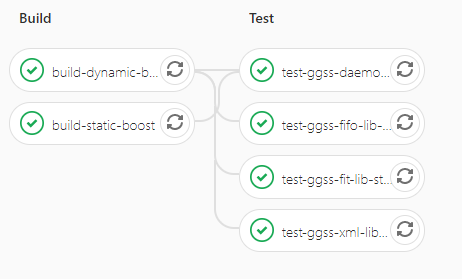
\includegraphics[width=0.75\textwidth]{resources/pipeline_example.png}
\caption{Example of CI pipeline used in the project.}
\end{figure}
\end{frame}


\begin{frame}[fragile]
\frametitle{CMake files refactoring}
\begin{itemize}
\item CMake files have been slightly refactored to improve readability by using macros and functions.
\item Doxygen and unit testing support have been added.
\end{itemize}
\begin{lstlisting}[language=c++, caption={New version of CMake used for building \emph{thread-lib}}]
set(CMAKE_MODULE_PATH "${GGSS_MISC_PATH}")
include(BuildLibrary)

ggss_build_library(
    TARGET_NAME "thread"
    DEPENDENCY_PREFIX "${CMAKE_CURRENT_SOURCE_DIR}/.."
    DEPENDENCIES "log" "sigslot"
)
\end{lstlisting}
\end{frame}


\begin{frame}[fragile]
\frametitle{Complex submodule structure handling - scripts}
\begin{itemize}
\item GGSS project tree contains a complex repository structure with many connections between components.
\item To make it easy to properly initialize project structure git submodules are being used.
\end{itemize}
\begin{lstlisting}[language=c++, caption={Initialize project structure with one command.}]
root@host:/# git clone ssh://git@gitlab.cern.ch:7999/atlas-trt-dcs-ggss/ggss-all.git && cd ggss-all && git submodule update --init --recursive
Cloning into '/CERN/ggss-all/ggss-dim-cs'...
Cloning into '/CERN/ggss-all/ggss-driver'...
Cloning into '/CERN/ggss-all/ggss-oper'...
Cloning into '/CERN/ggss-all/ggss-runner'...
Cloning into '/CERN/ggss-all/ggss-spector'...
Cloning into '/CERN/ggss-all/mca-n957'...
Cloning into '/CERN/ggss-all/ggss-dim-cs/external-dim-lib'...
Cloning into '/CERN/ggss-all/ggss-dim-cs/ggss-misc'...
Cloning into '/CERN/ggss-all/ggss-driver/external-n957-lib'...
Cloning into '/CERN/ggss-all/ggss-driver/ggss-misc'...
...(13 lines truncated)
\end{lstlisting}
\end{frame}

\begin{frame}[fragile]
\frametitle{Complex submodule structure handling - scripts}
\begin{itemize}
\item Using submodules requires to take care of commit hashes that are being linked as a submodule.
\item There may be a situation that "parent" repository is not using the latest version of "child" repository.
\end{itemize}
\begin{figure}
    \centering
    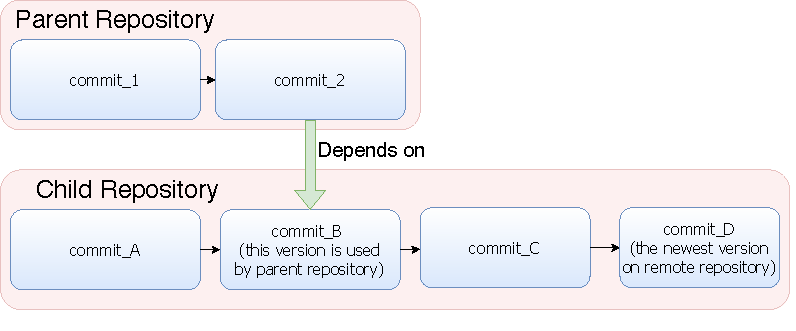
\includegraphics[width=0.8\textwidth]{resources/submodules_problem.pdf}
    \caption{Version of submodule differs from version used by parent.}
\end{figure}
\end{frame}

\begin{frame}[fragile]
\frametitle{Complex submodule structure handling - scripts}
\begin{itemize}
\item gitio script is responsible for updating all outdated links between parent and child repositories.
\item The goal is achieved by creating dependency tree of all available repositories.
\item Starting from the bottom of the tree submodules are being aligned (git commands: add, commit, push).
\end{itemize}
\begin{lstlisting}[language=c++, caption={Gitio in action.}]
root@host:/# python gitio.py -p ./ggss-all/
...(17 lines truncated)
INFO - Aligning ./ggss-all/mca-n957 repository
INFO - Aligning ./ggss-all/ggss-dim-cs repository
INFO - Aligning ./ggss-all/ggss-runner repository
INFO - Aligning ./ggss-all/ggss-spector repository
INFO - Aligning ./ggss-all/ggss-oper repository
INFO - Aligning ./ggss-all/ggss-driver repository
INFO - Aligning ./ggss-all repository
INFO - Aligning finished.
\end{lstlisting}
\end{frame}


\begin{frame}[fragile]
\frametitle{Automated versioning}
\begin{itemize}
\item Automated versioning system has been prepared to keep consistent rpm and release versions throughout whole project.
\item Every commit to main repository (ggss-all) is being analyzed. If commit message contains one of specified phrases, new release is being created.
\end{itemize}
\begin{figure}
    \centering
    
\includegraphics[width=0.8\textwidth]{resources/commit.PNG}
    \caption{New commit following eslint convention.}
\end{figure}
\begin{figure}
    \centering
    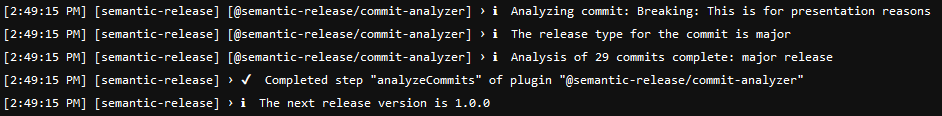
\includegraphics[width=0.8\textwidth]{resources/commit_message_analyze.PNG}
    \caption{Commit message analysis.}
\end{figure}

\end{frame}


\begin{frame}[fragile]
\frametitle{Automated versioning}
\begin{figure}
    \centering
    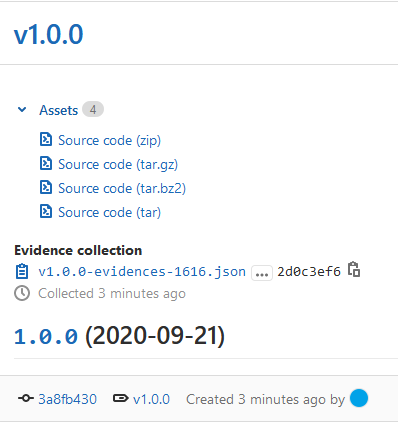
\includegraphics[width=0.45\textwidth]{resources/new_release.PNG}
    \caption{Newly created release.}
\end{figure}
\end{frame}


\begin{frame}[fragile]
\frametitle{Work in progress}
\begin{itemize}
    \item Hardware testing scripts refactoring and upgrade (yaml based scenarios).
    \item Gitio script improvements (interactive entry point, automated repository structure initialization).
    \item Custom artifacts (RPM package, compiled code, documentation) attached to releases.
    \item HV management commands refactoring (user-friendly format for SET and MON commands).
\end{itemize}
\end{frame}

\begin{frame}[c]
\hfill
\begin{center}
\large{
	Thanks for Your attention.
}
\hfill
\end{center}
\end{frame}

\end{document}